\documentclass{article}
\usepackage{tikz}

\usepackage[utf8]{inputenc}
\usepackage{color}
\usepackage{hyperref}

% für Listings
\usepackage{listings}
\lstset{numbers=left, numberstyle=\tiny, numbersep=5pt, keywordstyle=\color{black}\bfseries, stringstyle=\ttfamily,showstringspaces=false,basicstyle=\footnotesize,captionpos=b}
\lstset{
	frame=none,
	xleftmargin=2pt,
	stepnumber=1,
	numbers=left,
	numbersep=5pt,
	numberstyle=\ttfamily\tiny\color[gray]{0.3},
	belowcaptionskip=\bigskipamount,
	captionpos=b,
	escapeinside={*'}{'*},
	language=haskell,
	tabsize=2,
	emphstyle={\bf},
	commentstyle=\it,
	stringstyle=\mdseries\rmfamily,
	showspaces=false,
	keywordstyle=\bfseries\rmfamily,
	columns=flexible,
	basicstyle=\small\sffamily,
	showstringspaces=false,
	morecomment=[l]\%,
}

\newcommand{\cit}[2]{\footnote{#1, see~\cite{#2}}}

\newcommand{\citHughes}{\cit{John Hughes, Generalising Monads to Arrows}{hughes_arrows_98}}

\begin{document}
	\title{Parrows}
	
	\newpage
	\tableofcontents
	~
	\pagebreak
	
	\section{General Introduction}
Arrows were introduced in John Hughes paper as an alternative to Monads for API design.\citHughes In the paper Hughes describes that Arrows have one powerful additional property when compared to Monads for API design: Extensibility. In this paper we will show how this property can be used to add parallelism capabilities to different arrows.
	\section{Background}
\label{sec:background}
\subsection{Short introduction to parallel Haskells}
There are already several ways to write parallel programs in Haskell. As we will base our parallel arrows on existing parallel Haskells, we will now give a short introduction to the ones we use as backends in this paper.

In its purest form, parallel computation (on functions) can be looked at as the execution of some functions \inlinecode{a -> b} in parallel:

\begin{figure}[h]
%\begin{lstlisting}[frame=htrbl]
\begin{code}
parEvalN :: [a -> b] -> [a] -> [b]
\end{code}
%\end{lstlisting}
\caption{parEvalN's type signature}
\label{fig:parEvalNTypeSig}
\end{figure}
\begin{figure}[h]
	\includegraphics[scale=0.7]{images/parEvalN}
	\caption{Schematic illustration of parEvalN}
	\label{fig:parEvalN}
\end{figure}
\olcomment{make them to real figures? with environment, reference and such?}
Before we go into detail on how we can use this idea of parallelism for parallel Arrows, as a short introduction to parallelism in Haskell we will now implement \inlinecode{parEvalN} with several different parallel Haskells.

\subsubsection{Multicore Haskell}
Multicore Haskell \cite{Marlow2009,Trinder1999} is way to do parallel processing found in standard GHC.\footnote{Multicore Haskell on Hackage is available under \url{https://hackage.haskell.org/package/parallel-3.2.1.0}, compiler support is integrated in the stock GHC.} It ships with parallel evaluation strategies \cite{Trinder1998a,Marlow2010} for several types which can be applied with \inlinecode{using :: a -> Strategy a -> a}. For \inlinecode{parEvalN} this means that we can just apply the list of functions \inlinecode{[a -> b]} to the list of inputs \inlinecode{[a]} by zipping them with the application operator \inlinecode{\$}. We then evaluate this lazy list \inlinecode{[b]} according to a \inlinecode{Strategy [b]} with the \inlinecode{using :: a -> Strategy a -> a} operator. We construct this strategy with \inlinecode{parList :: Strategy a -> Strategy [a]} and \inlinecode{rdeepseq :: NFData a => Strategy a} where the latter is a strategy which evalutes to normal form. To ensure that programs that use \inlinecode{parEvalN} have the correct evaluation order, we annotate the computation with \inlinecode{pseq :: a -> b -> b} which forces the compiler to not reorder multiple \inlinecode{parEvalN} computations. This is particularly necessary in circular communication topologies like in the \inlinecode{torus} or \inlinecode{ring} skeleton that we will see in chapter \ref{sec:topology-skeletons} which resulted in deadlock scenarios when executed without \inlinecode{pseq} during testing for this paper.

\begin{lstlisting}[frame=htrbl]
parEvalN :: (NFData b) => [a -> b] -> [a] -> [b]
parEvalN fs as = let bs = zipWith ($) fs as in
	(bs `using` parList rdeepseq) `pseq` bs
\end{lstlisting}
\begin{figure}[h]
	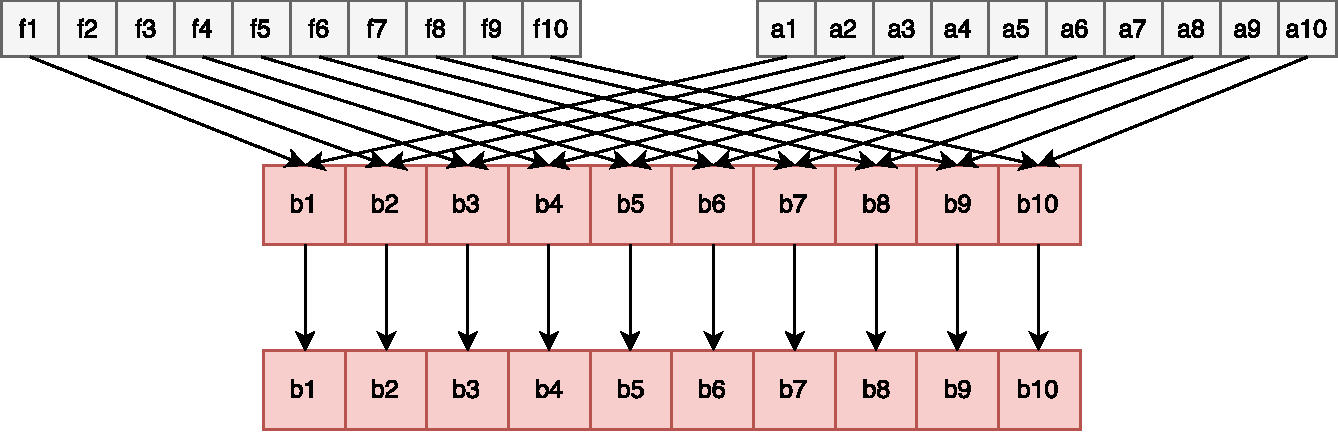
\includegraphics[scale=0.5]{images/parEvalNMulticore}
	\caption{Dataflow of the Multicore Haskell parEvalN version}
\end{figure} %$ %% formatting

\subsubsection{ParMonad}
The \inlinecode{Par} monad\footnote{It can be found in the \texttt{monad-par} package on hackage under \url{https://hackage.haskell.org/package/monad-par-0.3.4.8/}.} introduced by \citet{monad_par_paper_2011}, is a monad designed for composition of parallel programs.


Our parallel evaluation function \inlinecode{parEvalN} can be defined by zipping the list of \inlinecode{[a -> b]} with the list of inputs \inlinecode{[a]} with the application operator \inlinecode{\$} just like with Multicore Haskell. Then, we map over this not yet evaluated lazy list of results \inlinecode{[b]} with \inlinecode{spawnP :: NFData a => a -> Par (IVar a)} to transform them to a list of not yet evaluated forked away computations \inlinecode{[Par (IVar b)]}, which we convert to \inlinecode{Par [IVar b]} with \inlinecode{sequenceA}. We wait for the computations to finish by mapping over the \inlinecode{IVar b}'s inside the \inlinecode{Par} monad with \inlinecode{get}. This results in \inlinecode{Par [b]}. We finally execute this process with \inlinecode{runPar} to finally get \inlinecode{[b]} again.

\textbf{\textcolor{red}{explain problems with laziness here. Problems with torus}}

\begin{lstlisting}[frame=htrbl]
parEvalN :: (NFData b) => [a -> b] -> [a] -> [b]
parEvalN fs as = runPar $ 
	(sequenceA $ map (spawnP) $ zipWith ($) fs as) >>= mapM get
\end{lstlisting}
\begin{figure}[h]
	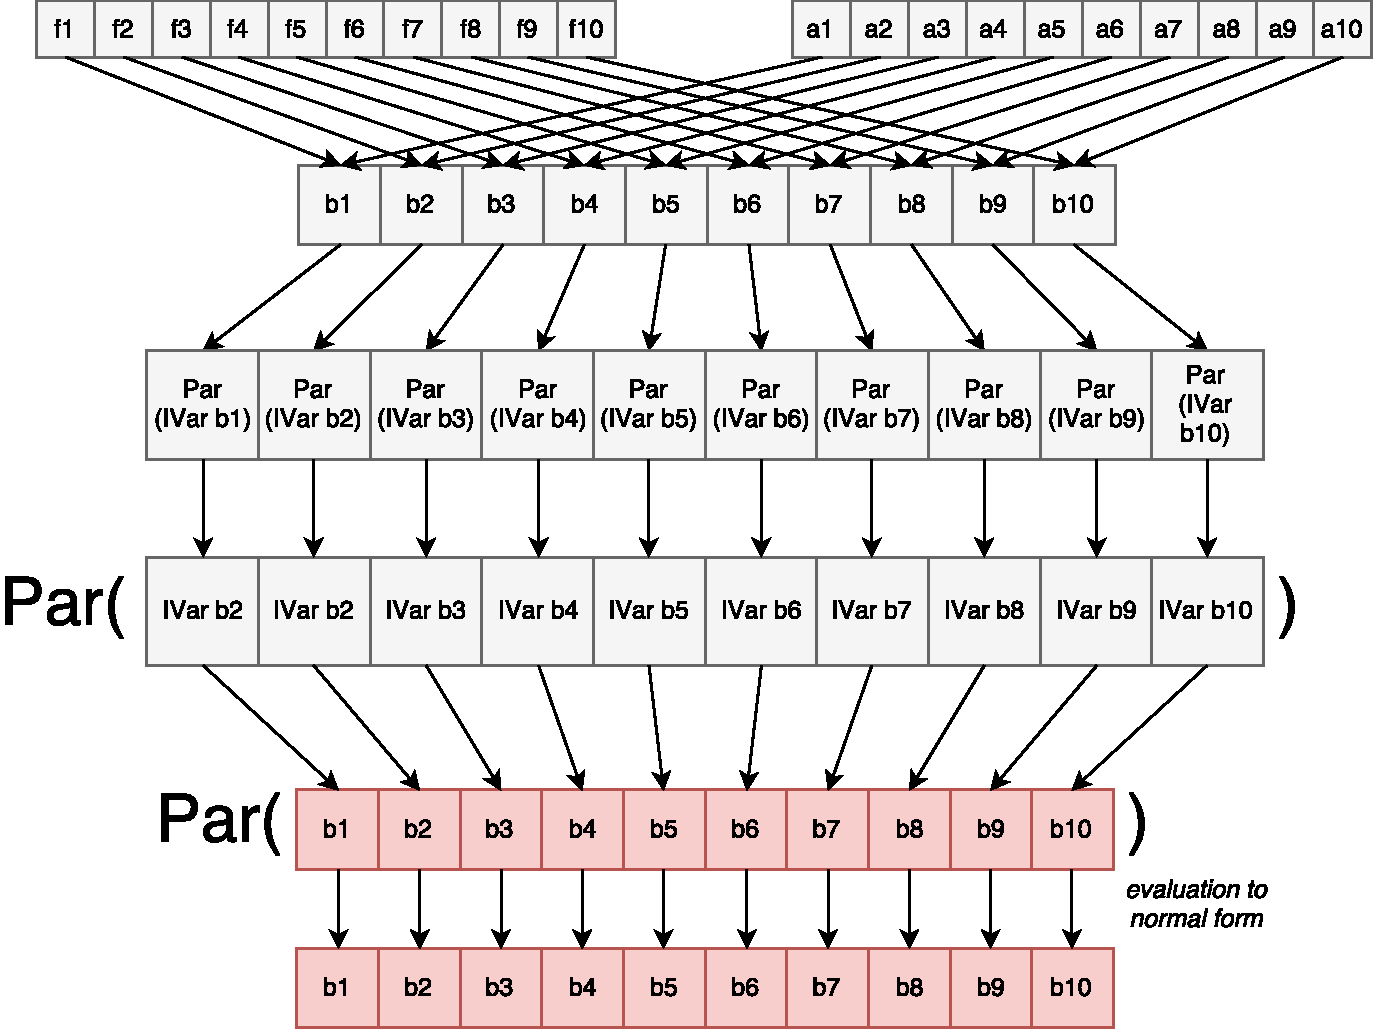
\includegraphics[scale=0.5]{images/parEvalNParMonad}
	\caption{Dataflow of the Par Monad parEvalN version}
\end{figure}

\subsubsection{Eden}
Eden \cite{eden,Loogen2012} is a parallel Haskell for distributed memory and comes with a MPI and a PVM backends.\footnote{See also \url{http://www.mathematik.uni-marburg.de/~eden/} and \url{https://hackage.haskell.org/package/edenmodules-1.2.0.0/}.} This means that it works on clusters as well so it makes sense to have a Eden-based backend for our new parallel Haskell flavour.

Eden was designed to work on clusters, but with a further simple backend it operates on multicores. However, in contrast to many other parallel Haskells, in Eden each process has its own heap. This seems to be a waste of memory, but with distributed programming paradigm and individual GC per process, Eden yields good performance results also on multicores \cite{arcs-dc,aswad2009low}.

While Eden also comes with a monad \inlinecode{PA} for parallel evaluation, it also ships with a completely functional interface that includes
%\\
%\inlinecode{spawnF :: (Trans a, Trans b) => [a -> b] -> [a] -> [b]}.
%\\
a \inlinecode{spawnF} function that
%This 
allows us to define \inlinecode{parEvalN} directly:

\begin{lstlisting}[frame=htrbl]
parEvalN :: (Trans a, Trans b) => [a -> b] -> [a] -> [b]
parEvalN = spawnF 
\end{lstlisting}
\begin{figure}[h]
	\includegraphics[scale=0.5]{images/parEvalNEden}
	\caption{Dataflow of the Eden parEvalN version}
\end{figure}

\paragraph{Eden TraceViewer.}
To comprehend the efficiency and the lack thereof in a parallel program, an inspection of its execution is extremely helpful. While some large-scale solutions exist \cite{Geimer2010}, the parallel Haskell community mainly utilises the tools Threadscope \cite{Wheeler2009} and Eden TraceViewer\footnote{See ..... on hackage for the last available version of Eden TraceViewer. There was an effort to implement the TraceViewer using modern web technologies \cite{traceviewer-web}.} \cite{Berthold2007a}. In the next sections we will present some \emph{traces}, the post-mortem process diagrams of Eden processes and their activity.

In a trace, the $x$ axis shows the time, the $y$ axis enumerates the machines and processes. A~trace shows a running process in green, a blocked process is red. If the process is \enquote{runnable}, \ie it may run, but does not, it is yellow. The typical reason for then is GC. An inactive machine where no processes are started yet, or all are already terminated, is shows as a blue bar. A~comminication from one process to another is represented with a black arrow. A~stream of communications, \eg a transmitted list is shows as a dark shading between sender and receiver processes.

\olcomment{show example trace or refer to a trace in later figures}


%%% Local Variables:
%%% mode: latex
%%% TeX-master: "main"
%%% End:

	\begin{figure}[t]
\centering
\begin{code}
class Arrow arr where
  arr :: (a -> b) -> arr a b
  (>>>) :: arr a b -> arr b c -> arr a c
  first :: arr a b -> arr (a,c) (b,c)

instance Arrow (->) where
	arr f = f
	f >>> g = g . f
	first f = \(a, c) -> (f a, c) 

data Kleisli m a b = Kleisli { run :: a -> m b }

instance Monad m => Arrow (Kleisli m) where
	arr f = Kleisli (return . f)
	f >>> g = Kleisli (\a -> f a >>= g)
	first f = Kleisli (\(a,c) -> f a >>= \b -> return (b,c))
\end{code}
\vfill
\caption{The definition of the |Arrow| type class and its two most typical instances.}
\label{fig:ArrowDefinition}
\end{figure}

\begin{figure}[t]
\centering
\parbox[c][17em]{0.49\linewidth}{%
\vfill
\centering
	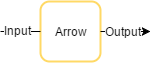
\includegraphics{images/arrow}
\vfill
%	\caption{Schematic depiction of an Arrow.}
%\label{fig:arrow-sch}
}
\parbox[c][17em]{0.49\linewidth}{%
\vfill
\centering
	{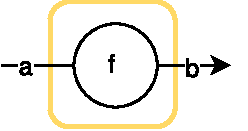
\includegraphics[scale=0.6]{images/arr}}
	{\includegraphics[scale=0.6]{images/compose}}
	{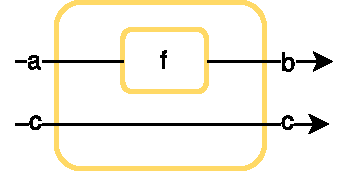
\includegraphics[scale=0.6]{images/first}}
\vfill
%\caption{Schematic depiction of |Arrow| combinators |arr|, |>>>| and |first|.}
%\label{fig:arrows-viz}
}
\caption{Schematic depiction of  an Arrow (left) and its basic
  combinators |arr|, |>>>| and |first| (right).}
\label{fig:arrow-sch}
\label{fig:arrows-viz}
\end{figure}

\subsection{Arrows}
\label{sec:arrows}
Arrows were introduced by \citet{HughesArrows} as a general interface for computation. An Arrow |arr a b| represents  a computation that converts an input |a| to an output |b|. This is defined in the |Arrow| type class shown in Fig.~\ref{fig:ArrowDefinition}.
%
To lift an ordinary function to an Arrow, |arr| is used, analogous to the monadic |return|. Similarly, the composition operator |>>>| is analogous to the monadic composition |>>=| and combines two arrows |arr a b| and |arr b c| by \enquote{wiring} the outputs of the first to the inputs to the second to get a new arrow |arr a c|. Lastly, the |first| operator takes the input Arrow |arr a b| and converts it into an arrow on pairs |arr (a, c) (b, c)| that leaves the second argument untouched. It allows us to to save input across arrows. Figure~\ref{fig:arrows-viz} shows a graphical representation of these basic Arrow combinators.
The most prominent instances of this interface are regular functions |(->)|
and the Kleisli type (Fig.~\ref{fig:ArrowDefinition}), which wraps monadic functions, e.g.  |a -> m b| (with |m| being a Monad).

\begin{figure}[h]
	\centering
	\begin{tabular}{cc}
		% \subcaptionbox
{\label{t1}}{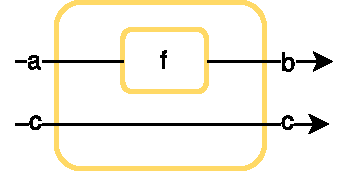
\includegraphics[width = 1.5in]{images/first}} &
		% \subcaptionbox
{\label{fig:secondImg}}{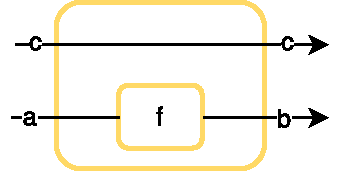
\includegraphics[width = 1.5in]{images/second}} \\
|first| & |second| \\
\midrule
		% \subcaptionbox
{}{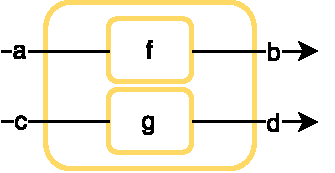
\includegraphics[width = 1.5in]{images/starstarstar}} &
		% \subcaptionbox
{}{\includegraphics[width = 1.5in]{images/andandand}}\\
|(***)|\label{fig:***Img} & |(&&&)| \label{fig:&&&Img} \\
	\end{tabular}
	\caption{Visual depiction of syntactic sugar for Arrows.}
	\label{fig:syntacticSugarArrows}
\end{figure}
Hughes also defined some syntactic sugar (Fig.~\ref{fig:syntacticSugarArrows}): |second|, |***| and |&&&|. 
|second| is the mirrored version of |first| (Appendix~\ref{utilfns}).
|***| combines |first| and |second| to handle two inputs in one arrow, and is defined as follows:
% \begin{figure}[h]
\begin{code}
(***) :: Arrow arr => arr a b -> arr c d -> arr (a, c) (b, d)
f *** g = first f >>> second g
\end{code}
% \caption{The (***) combinator}
% \label{fig:***}
% \end{figure}
The |&&&| combinator, which constructs an Arrow that outputs two different values like |***|, but takes only one input, is:
% \begin{figure}[h]
\begin{code}
(&&&) :: Arrow arr => arr a b -> arr a c -> arr a (b, c)
f &&& g = arr (\a -> (a, a)) >>> (f *** g)
\end{code}
% \caption{The (\&\&\&) combinator}
% \label{fig:&&&}
% \end{figure}
A~first short example given by Hughes on how to use arrows is addition with arrows:
%|add| over arrows, which can be seen in Fig.~\ref{fig:addArrows}.
% \begin{figure}[h]
\begin{code}
add :: Arrow arr => arr a Int -> arr a Int -> arr a Int
add f g = (f &&& g) >>> arr (\(u, v) -> u + v)
\end{code}
% \caption{Add over arrows}
% \label{fig:addArrows}
% \end{figure}
% The benefit of using the |Arrow| typeclass is that any type which is shown to be an arrow can be used in conjunction with this newly created |add| combinator. Even though this example is quite simple, the power of the arrow interface immediately is clear: If a type is an arrow, it can automatically used together with every library that works on arrows. Compared to simple Monads, this enables us to write code that is more extensible, without touching the internals of the specific arrows.
% \\\\
% \textit{Note: In the definitions Hughes gave in his paper, the notation |a b c| for an arrow from |b| to |c| is used. We use the equivalent definition |arr a b| for an arrow from |a| to |b| instead, to make it easier to find the arrow type in type signatures.}
%

The more restrictive interface of Arrows allows for more elaborate composition and transformation combinators---a Monad can be \emph{anything}, an Arrow is a process of doing something, a \emph{computation}. This is exactly one of the key challenges in parallel computing.


%%% Local Variables:
%%% mode: latex
%%% TeX-master: "main"
%%% End:

	\pagebreak
	\begin{thebibliography}{100}
	
	\bibitem{hughes_arrows_98} Generalising Monads to Arrows
	\url{https://jcp.org/en/jsr/detail?id=220}, November 10, 1998
	
	\bibitem{marlow_parconc} Sample code for Simon Marlow's book "Parallel and Concurrent Programming in Haskell"
	\url{https://github.com/simonmar/parconc-examples}, retrieved on 01/12/2017
\end{thebibliography}
\end{document}